\documentclass[14pt,aspectratio=169,hyperref={pdftex,unicode},xcolor=dvipsnames]{beamer}
\usepackage[english,russian]{babel}
\usepackage[utf8x]{inputenc}
\usepackage[T2A]{fontenc}
\usepackage{cmap}
\usepackage{paratype}
\usepackage{minted} % для примеров кода (требует параметра -shell-escape)

\usepackage{hyperref}
\usepackage{xurl}

\usepackage{makecell}

\usepackage{comment}

% ===============================================

\renewcommand{\le}{\leqslant}
\renewcommand{\ge}{\geqslant}

\newcommand{\fakesc}[1]{\uppercase{{\footnotesize #1}}}
\renewcommand{\textsc}{\fakesc}

% ===============================================

\usetheme{metropolis}
\usefonttheme[]{professionalfonts}  % запрещаем beamer'у перезаписывать мат. шрифты
\metroset{numbering=fraction}
\metroset{subsectionpage=progressbar}

\setbeamercolor{frametitle}{fg=black}
\setbeamertemplate{frametitle}
{
 \vspace{3mm}\insertframetitle\par
}
\setbeamertemplate{title separator}{}
\setbeamertemplate{footnote separator}{}

% \usebackgroundtemplate{
\includegraphics[width=\paperwidth,height=\paperheight]{./common/background_white.jpg}}

\logo{\vspace{-1.2cm}
\includegraphics[width=6mm]{./common/short-v.pdf}\hspace*{1.08\textwidth}}

\institute
{
  \begin{columns}
    \begin{column}{1.5cm}
    
\includegraphics[height=15mm,keepaspectratio]{./common/math-cs.pdf}
    \end{column}
    \begin{column}{4cm}
          Факультет математики и компьютерных наук СПбГУ
    \end{column}
  \end{columns}
}


\begin{document}



\begin{frame}[plain]
  \begin{center}
    \textbf{Степан Остапенко}

    {\Large\textbf{Проверка выполнимости SMT-формул с помощью нейронных сетей}}

    Выпускная квалификационная работа

    {\small Научный руководитель: Д.\,С.\,Шалымов}

    13.06.2024
  \end{center}


  \begin{columns}
    \begin{column}{1cm}
    
\includegraphics[height=15mm,keepaspectratio]{./common/math-cs.pdf}
    \end{column}
    \begin{column}{10cm}
      \small
          Факультет математики и~компьютерных наук СПбГУ\\
          Программа <<Современное программирование>>
    \end{column}
  \end{columns}
\end{frame}



\begin{frame}{Введение в предметную область}

\begin{gather*}
  ({\color{red}x}^2 + {\color{magenta}y} - {\color{blue}z}^2 = 2) \wedge ({\color{red}x}^2 + 2{\color{magenta}y} - 3{\color{blue}z}^2 \le 2) \wedge ({\color{red}x}^2 + 2{\color{magenta}y} - 4{\color{blue}z}^2 \ge 1),
\end{gather*}

\begin{center}
где ${\color{red}x}, {\color{magenta}y}, {\color{blue}z} \in \mathbb{Z} \ \longrightarrow \ {\color{red}x} = 1, {\color{magenta}y} = 2, {\color{blue}z} = -1$.
\end{center}

\begin{itemize}
  \item $\mathbb{B}$ --- \texttt{true}, \texttt{false}, логические операции;
  \item $\mathbb{Z}$ --- целые числа, арифметика, сравнения;
  \item $\mathbb{R}$ --- вещественные числа, арифметика, сравнения;
  \item \texttt{BitVec} --- битовые векторы, логические и арифметические операции;
\end{itemize}

\end{frame}



\begin{frame}{Зачем это нужно}

\begin{minipage}{0.5\textwidth}

\textbf{Применения}
\begin{itemize}
  \item составление расписания и планирование,
  \item верификация АО и ПО,
  \item вывод типов,
  \item {\color{magenta}символьное исполнение},
  \item статический анализ программ.
\end{itemize}

\end{minipage}%
\begin{minipage}{0.5\textwidth}

\begin{figure}[ht]
\begin{center}
  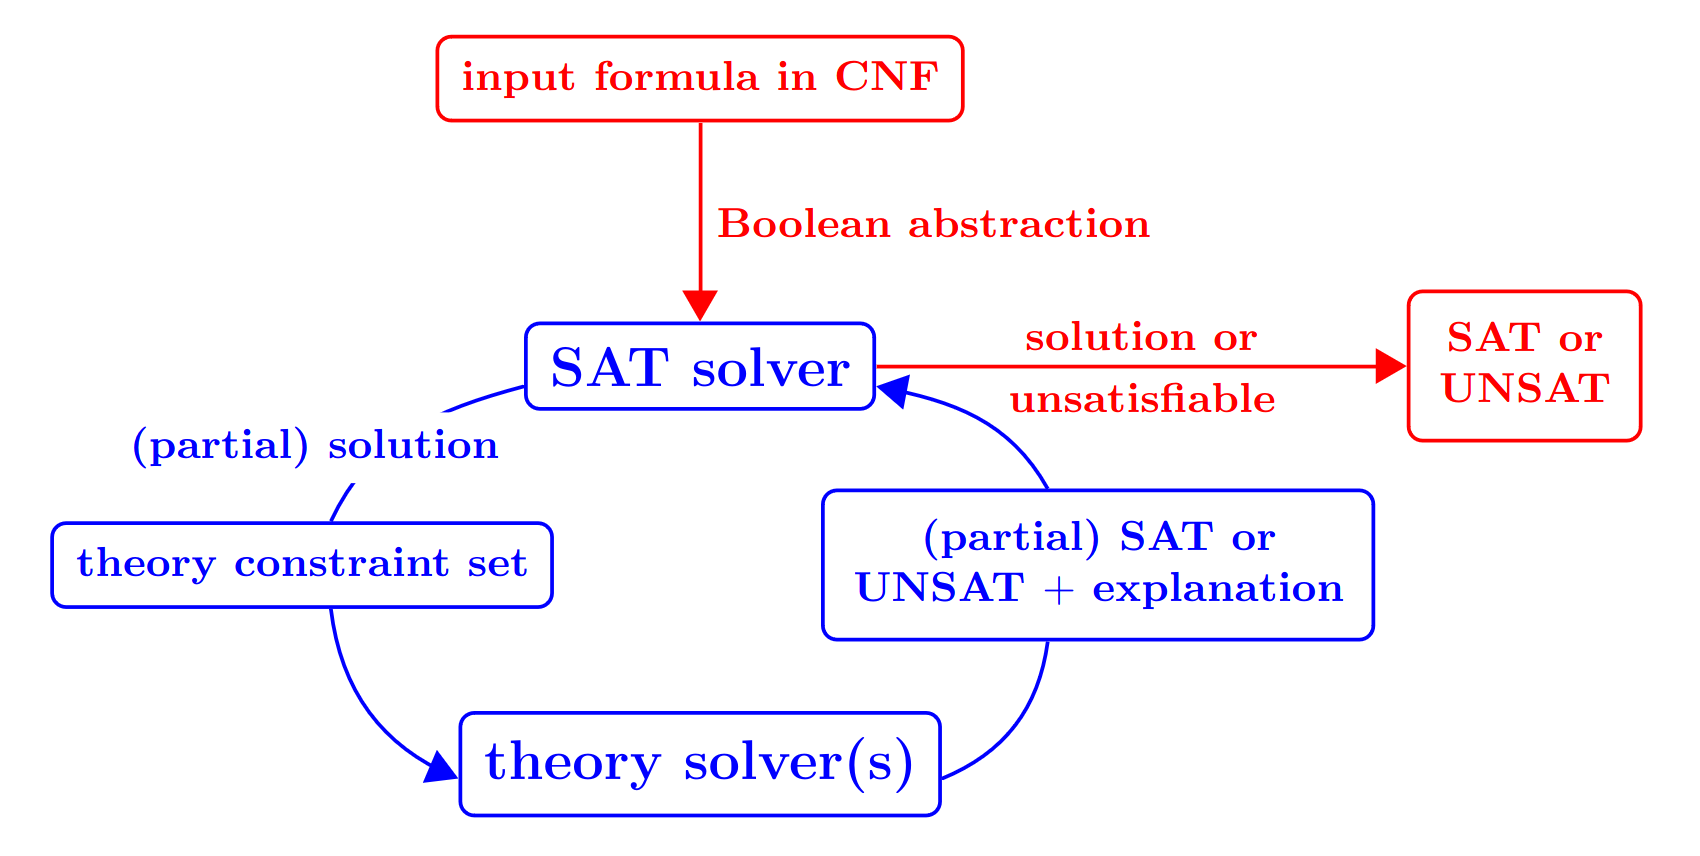
\includegraphics[scale=0.125]{./assets/smt-solver-working-scheme.png}
  \caption{Схема SMT-решателя \cite{smt-solver-working-scheme}.}
\end{center}
\end{figure}

\end{minipage}

\end{frame}



\begin{frame}{Постановка задачи}

\begin{center}
  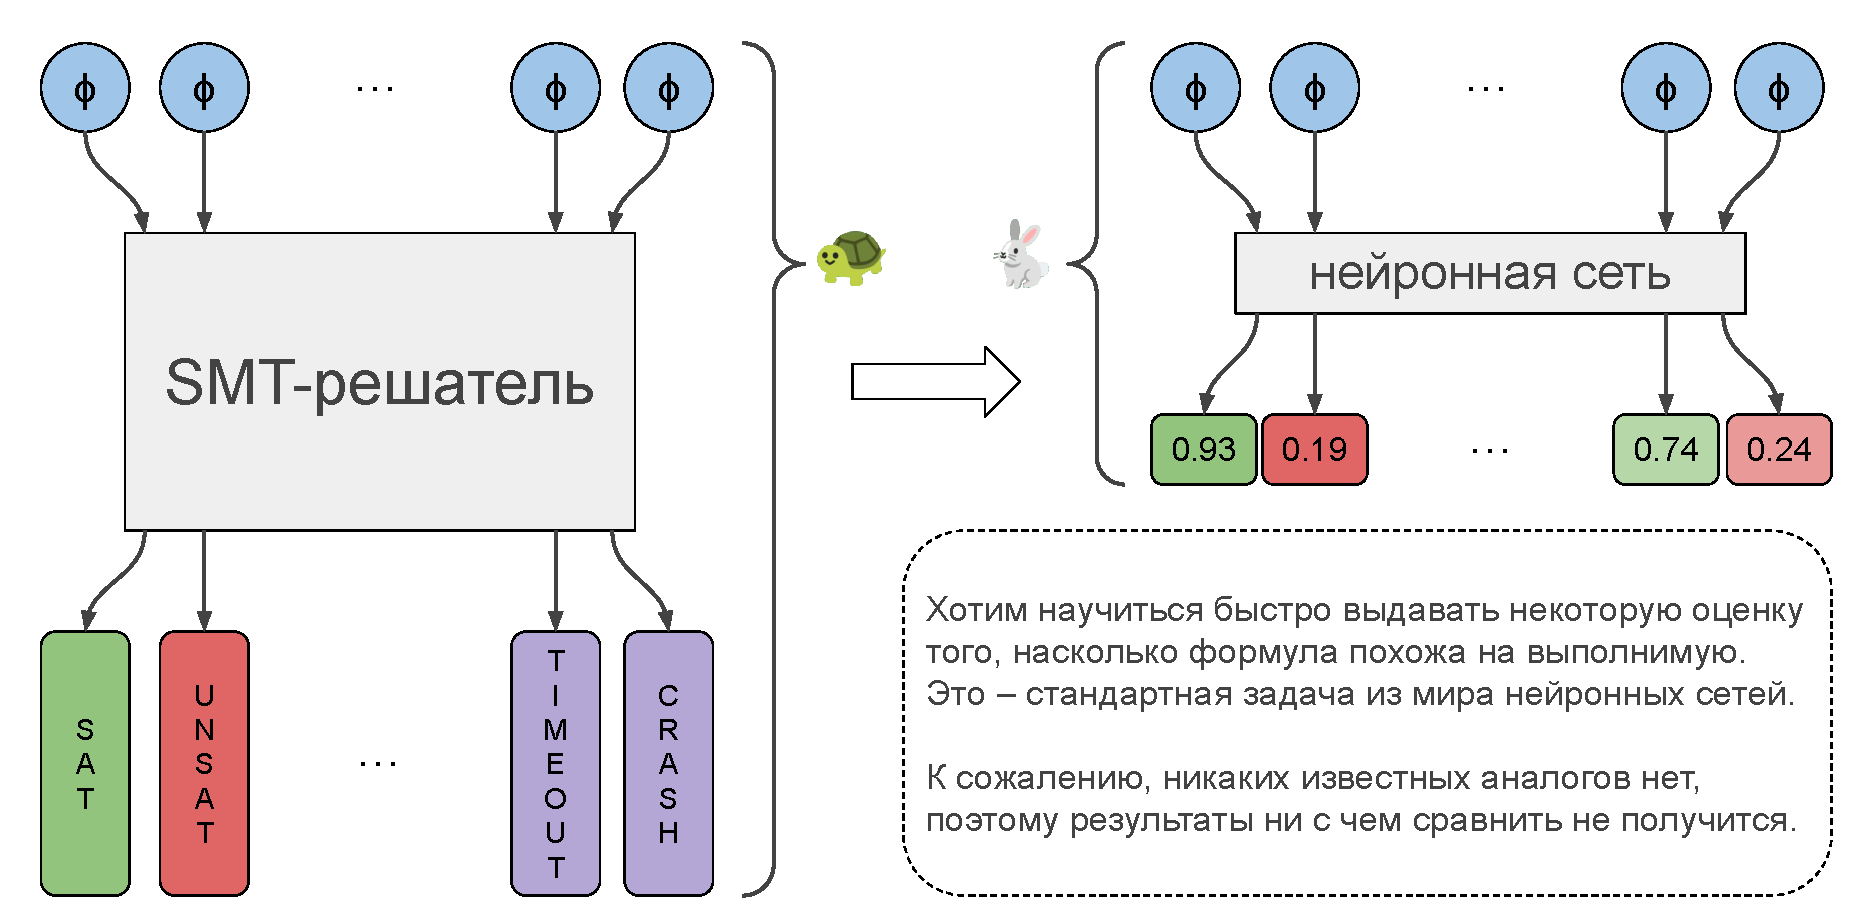
\includegraphics[scale=0.4]{./assets/problem-statement.pdf}
\end{center}

\end{frame}



\begin{frame}{Данные для обучения и оценки качества}

\begin{minipage}{0.5\textwidth}

\textbf{\texttt{SMT-COMP}} \cite{smt-comp-2023-benchmarks}

\end{minipage}%
\begin{minipage}{0.5\textwidth}

\textbf{\texttt{USVM}} \cite{usvm-github}

\end{minipage}

\begin{minipage}{0.5\textwidth}

\begin{center}
  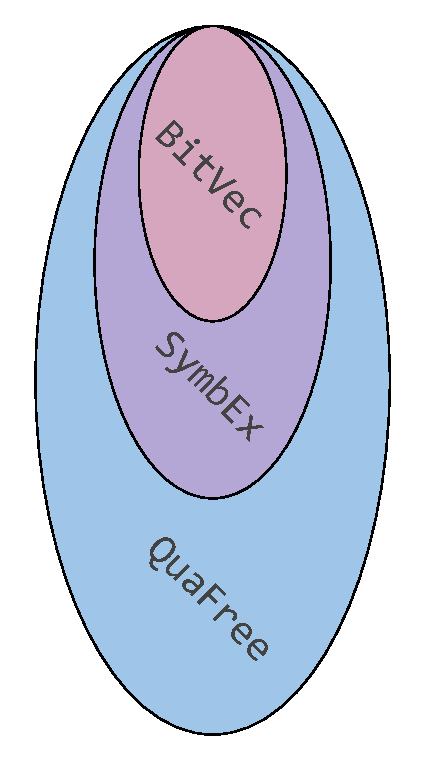
\includegraphics[scale=0.45]{./assets/smt-comp-datasets.pdf}
\end{center}

\end{minipage}%
\begin{minipage}{0.5\textwidth}

Наборы данных, состоящие из формул, возникших в процессе работы символьного движка:

\begin{itemize}
  \item обучающий набор --- запуск движка на нём же;
  \item 18 валидационных --- запуск движка на разных проектах на JVM-языках.
\end{itemize}

\end{minipage}

\end{frame}



\begin{frame}{Метрики}

\begin{figure}[ht]
\begin{center}
  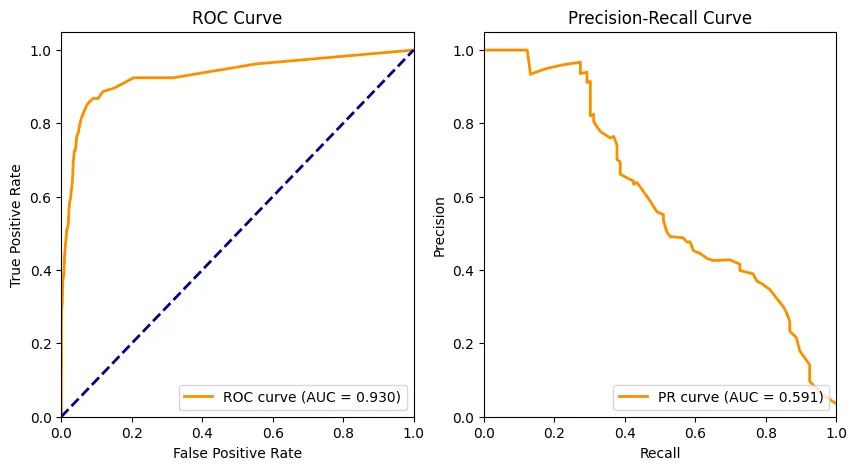
\includegraphics[scale=0.35]{./assets/roc-auc-vs-au-prc.jpg}
  \caption{Площадь под ROC-кривой и площадь под PR-кривой \cite{roc-auc-and-avg-prc}.}
\end{center}
\end{figure}

% todo: перерисовать картинку

\end{frame}



\begin{frame}{Архитектура}

\begin{minipage}{0.5\textwidth}

\begin{center}
  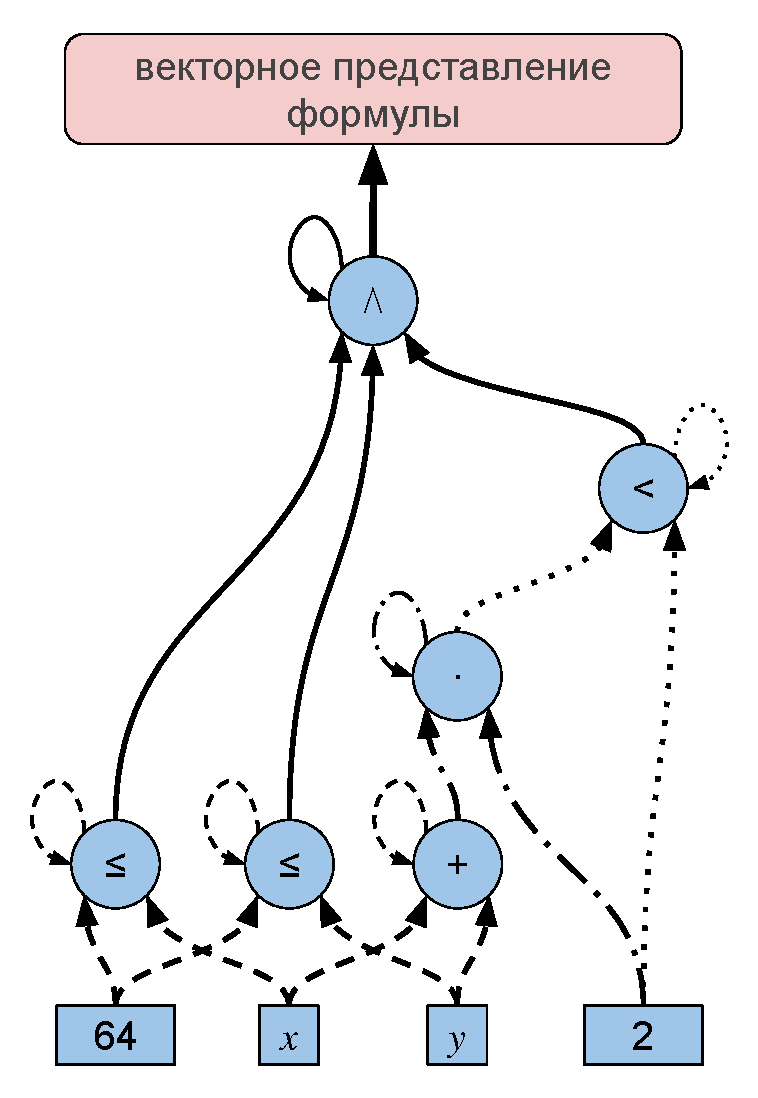
\includegraphics[scale=0.37]{./assets/formula-ast-talk.pdf}
\end{center}

\end{minipage}%
\begin{minipage}{0.5\textwidth}

В качестве графа вычислений берём AST формулы, превращённое в ациклический граф.

\medskip

Слева пример для формулы \\ {\small $(64 \le x) \wedge (64 \le y) \wedge ((x + y) \cdot 2 < 2)$}

\end{minipage}

\end{frame}



\begin{frame}{Архитектура}

\begin{minipage}{0.5\textwidth}

\begin{center}
  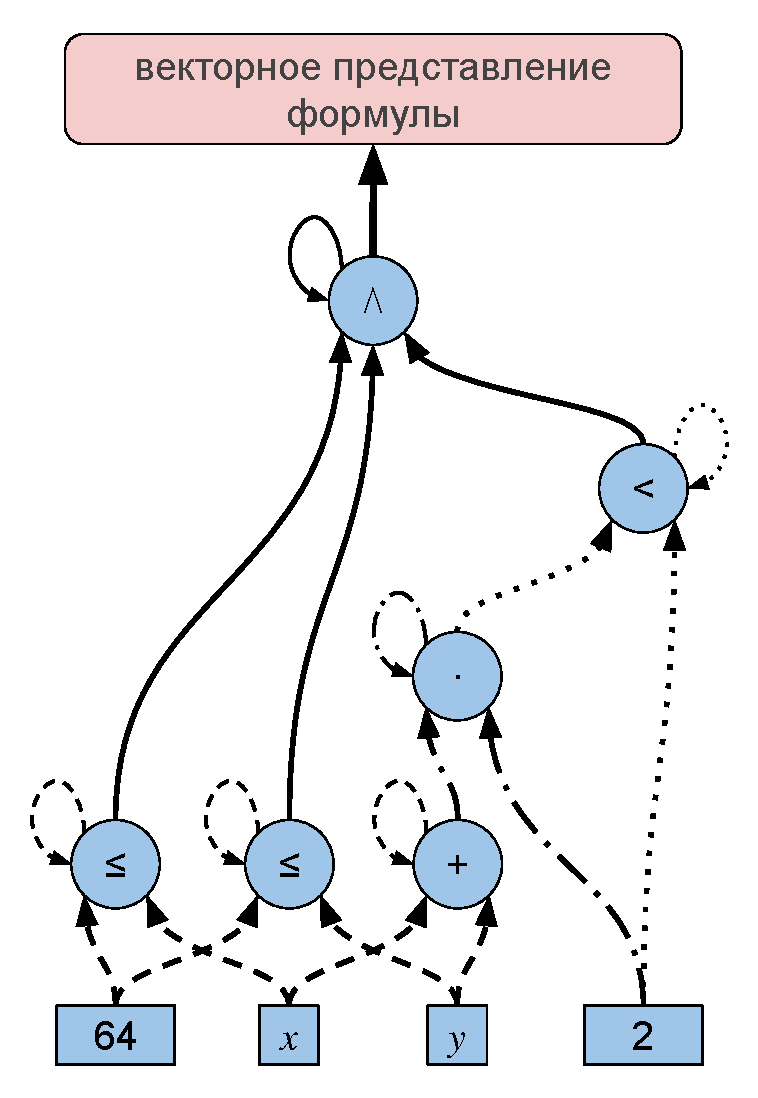
\includegraphics[scale=0.37]{./assets/formula-ast-talk.pdf}
\end{center}

\end{minipage}%
\begin{minipage}{0.5\textwidth}

\begin{center}
  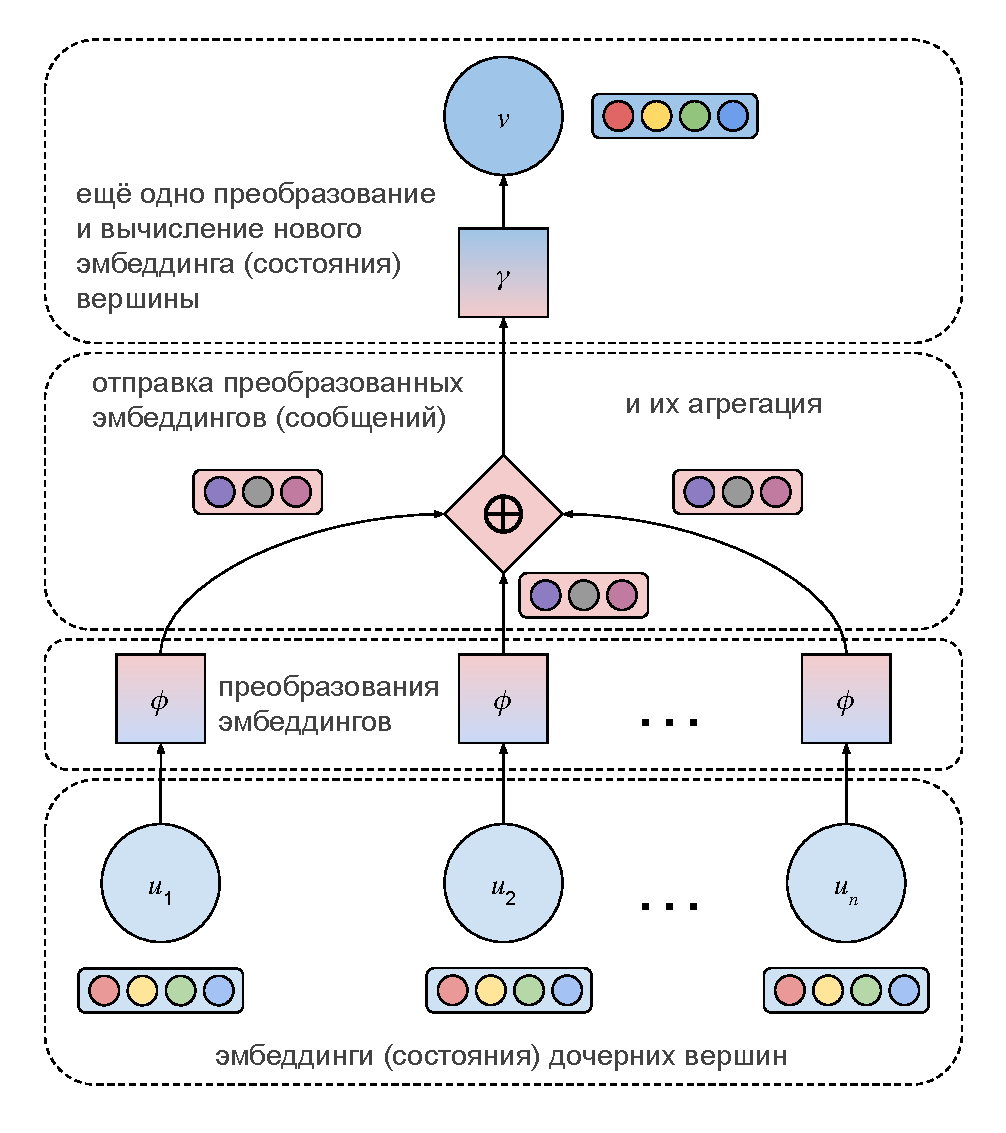
\includegraphics[scale=0.35]{./assets/message-passing-nn-talk.pdf}
\end{center}

\end{minipage}

\end{frame}



\begin{frame}

\begin{center}
  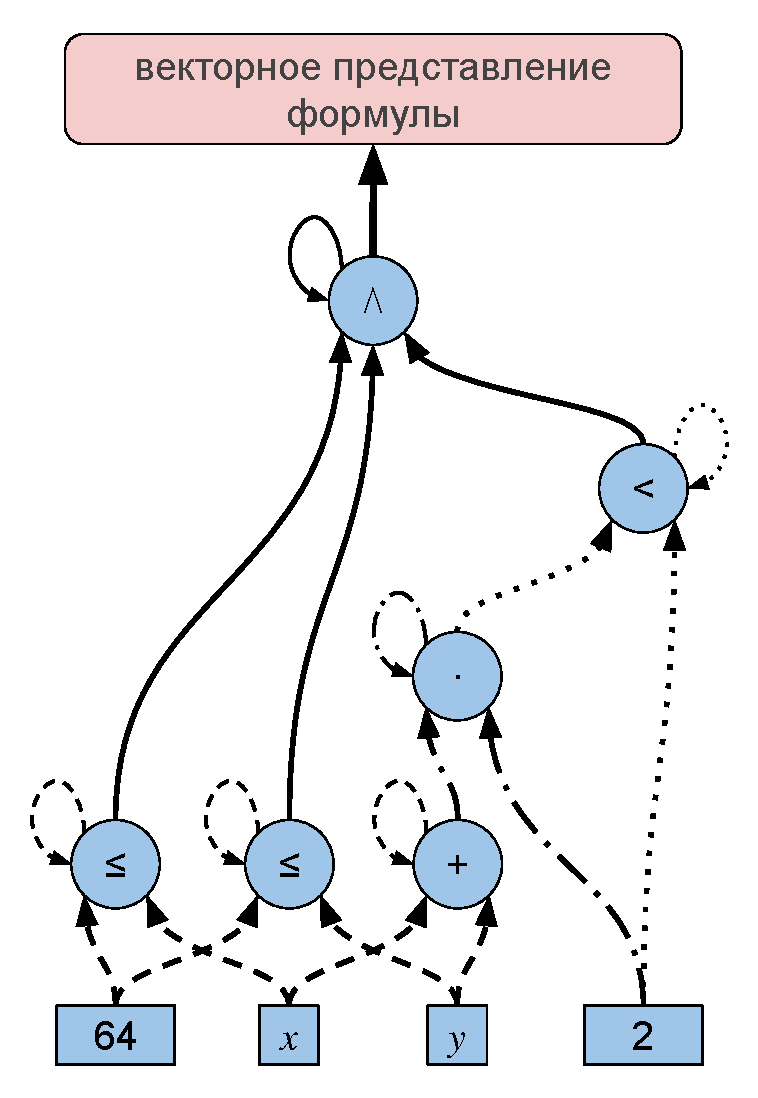
\includegraphics[scale=0.45]{./assets/formula-ast-talk.pdf}
\end{center}

\end{frame}



\begin{frame}[noframenumbering]

\begin{center}
  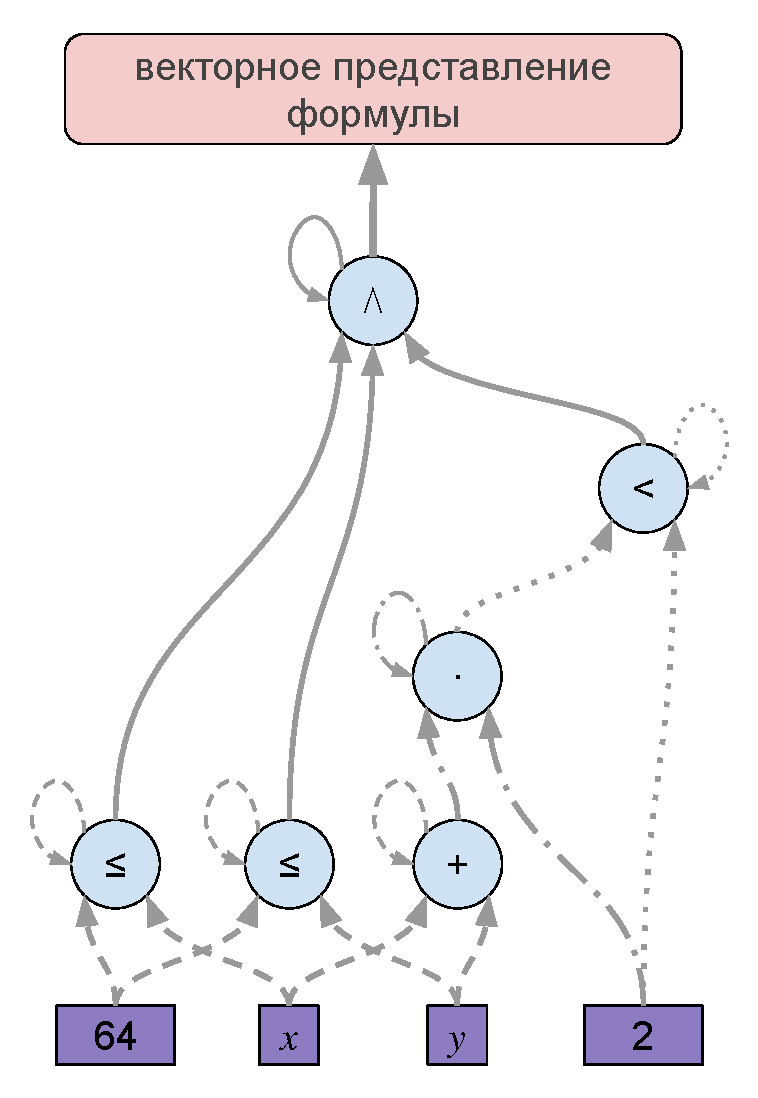
\includegraphics[scale=0.45]{./assets/formula-ast-talk-0.pdf}
\end{center}

\end{frame}



\begin{frame}[noframenumbering]

\begin{center}
  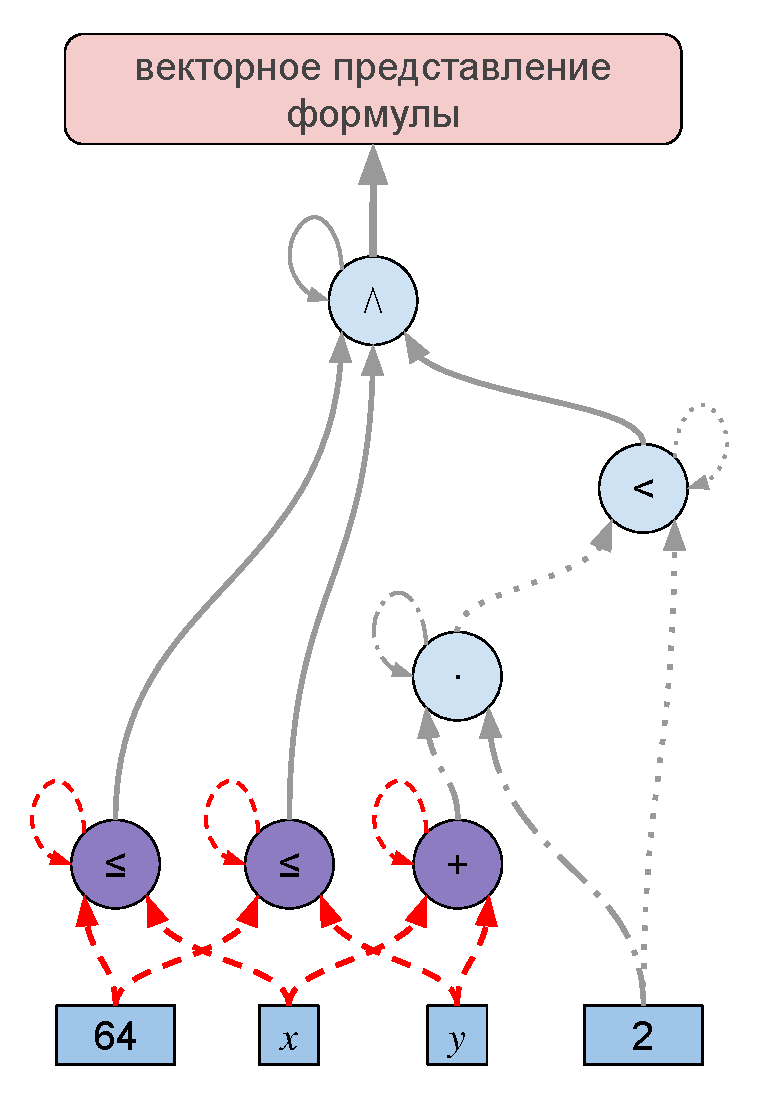
\includegraphics[scale=0.45]{./assets/formula-ast-talk-1.pdf}
\end{center}

\end{frame}



\begin{frame}[noframenumbering]

\begin{center}
  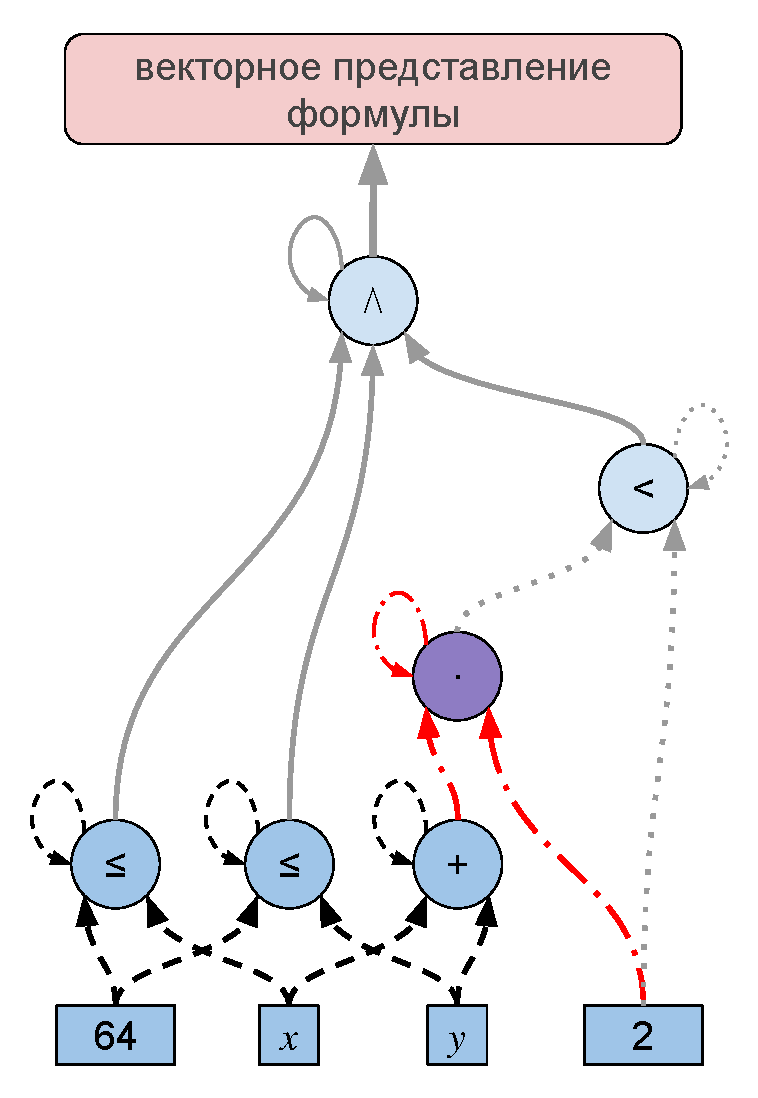
\includegraphics[scale=0.45]{./assets/formula-ast-talk-2.pdf}
\end{center}

\end{frame}



\begin{frame}[noframenumbering]

\begin{center}
  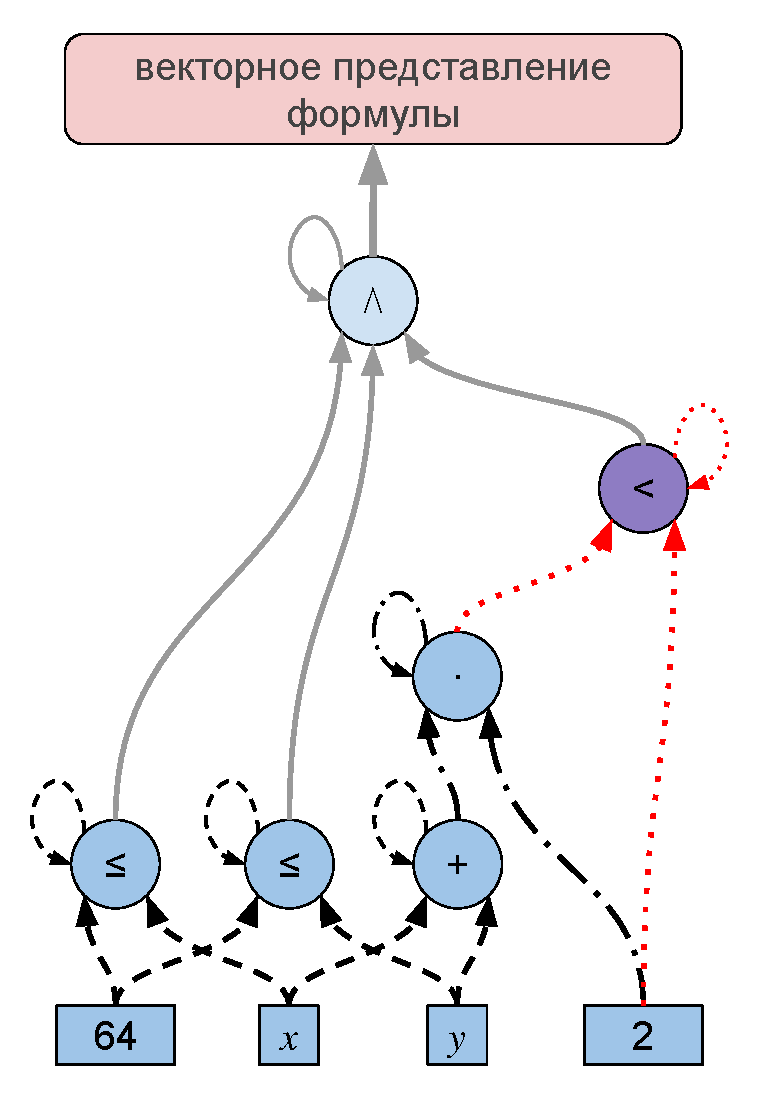
\includegraphics[scale=0.45]{./assets/formula-ast-talk-3.pdf}
\end{center}

\end{frame}



\begin{frame}[noframenumbering]

\begin{center}
  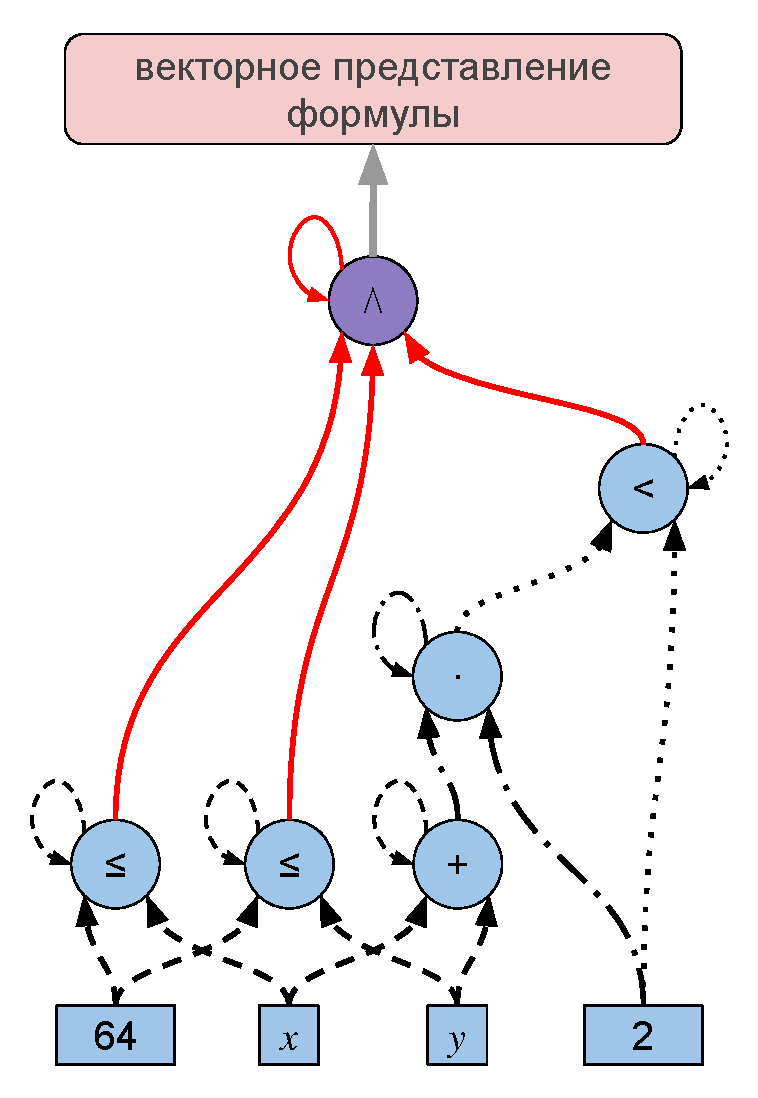
\includegraphics[scale=0.45]{./assets/formula-ast-talk-4.pdf}
\end{center}

\end{frame}



\begin{frame}[noframenumbering]

\begin{center}
  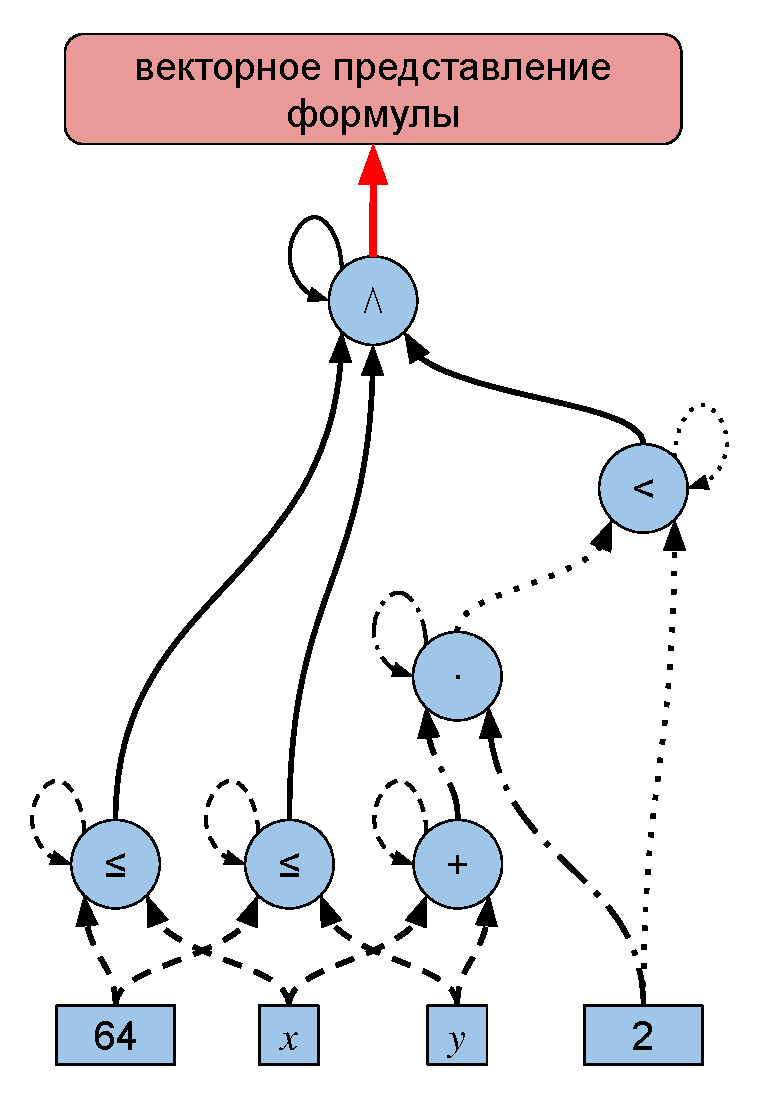
\includegraphics[scale=0.45]{./assets/formula-ast-talk-5.pdf}
\end{center}

\end{frame}



\begin{frame}[noframenumbering]

\begin{center}
  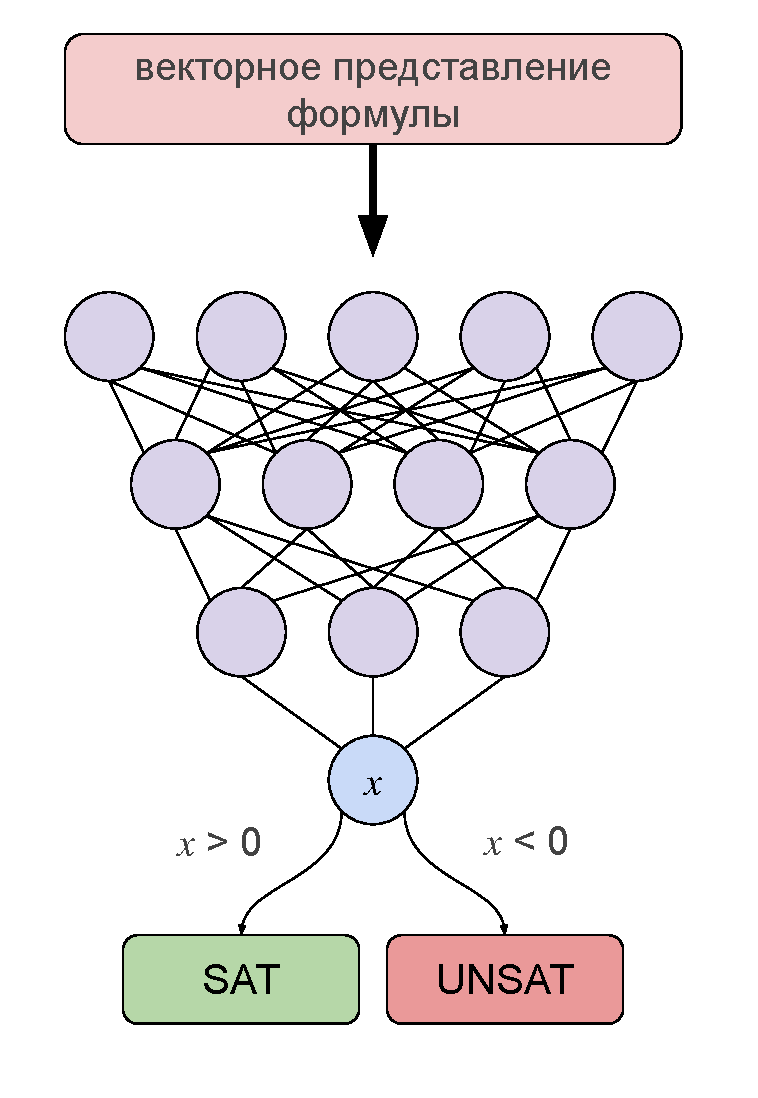
\includegraphics[scale=0.45]{./assets/formula-decoder.pdf}
\end{center}

\end{frame}



\begin{frame}{Как собрать детей по-быстрому?}

SAGE Convolution \cite{sage-conv-paper}:

\begin{equation*}
  x_v' = \sigma \left(W_3 \cdot \left(W_1 \cdot x_v + W_2 \cdot \underset{u \in \mathcal{N}(v)}{\text{\textsc{mean}}} x_u \right) + b \right)
\end{equation*}

\end{frame}



\begin{frame}{Как собрать детей по-быстрому?}

Transformer Convolution \cite{transformer-conv-paper}:

\begin{equation*}
  \alpha_{u} = \underset{u \in \mathcal{N}(v)}{\text{\textsc{softmax}}} \left[\frac{(W_3 \cdot x_v)^T (W_4 \cdot x_u)}{\sqrt d} \right]
\end{equation*}

\begin{equation*}
  x_v' = W_1 \cdot x_v + \sum_{u \in \mathcal{N}(v)} \alpha_u W_2 \cdot x_u
\end{equation*}

\end{frame}



\begin{frame}{Начальные состояния}

Проблема --- откуда взять начальные состояния?

\begin{itemize}
  \item Замена $m$, $k$, $n$ $\rightarrow$ \texttt{Var[Int]}; \hfill $2.8$, $2.4$, $3.0$ $\rightarrow$ \texttt{Val[Real]};
\end{itemize}

\vspace{1mm}\hrule\vspace{1mm}

\begin{minipage}{0.5\textwidth}

\textit{Для переменных:}

\begin{itemize}
  \item Случайные выученные векторы;
  \item Позиционное кодирование;
\end{itemize}

\end{minipage}%
\begin{minipage}{0.5\textwidth}

\textit{Для констант:}

\begin{itemize}
  \item Векторы с учётом групп (бинов) \cite{embeddings-for-numerical-features-paper};
  \item Преобразование с Fourier Feature Mapping \cite{embeddings-for-numerical-features-paper};
\end{itemize}

\end{minipage}

\end{frame}



\begin{frame}{Результаты SAGE Convolution (\texttt{SMT-COMP})}

\begin{minipage}{0.5\textwidth}

\begin{figure}[ht]
\begin{center}
  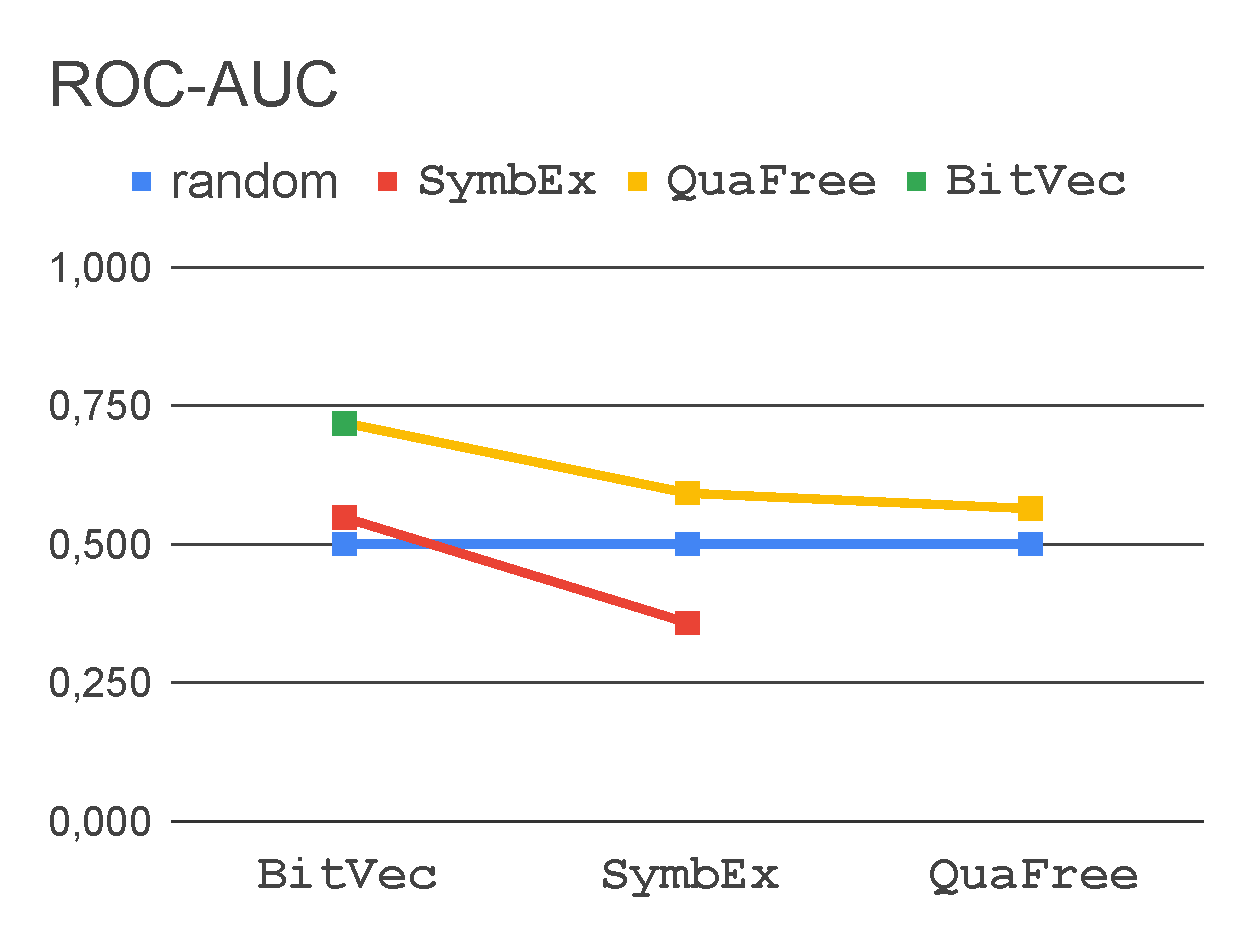
\includegraphics[scale=0.33]{./assets/smt-comp-roc-auc.pdf}
\end{center}
\end{figure}

\end{minipage}%
\begin{minipage}{0.5\textwidth}

\begin{figure}[ht]
\begin{center}
  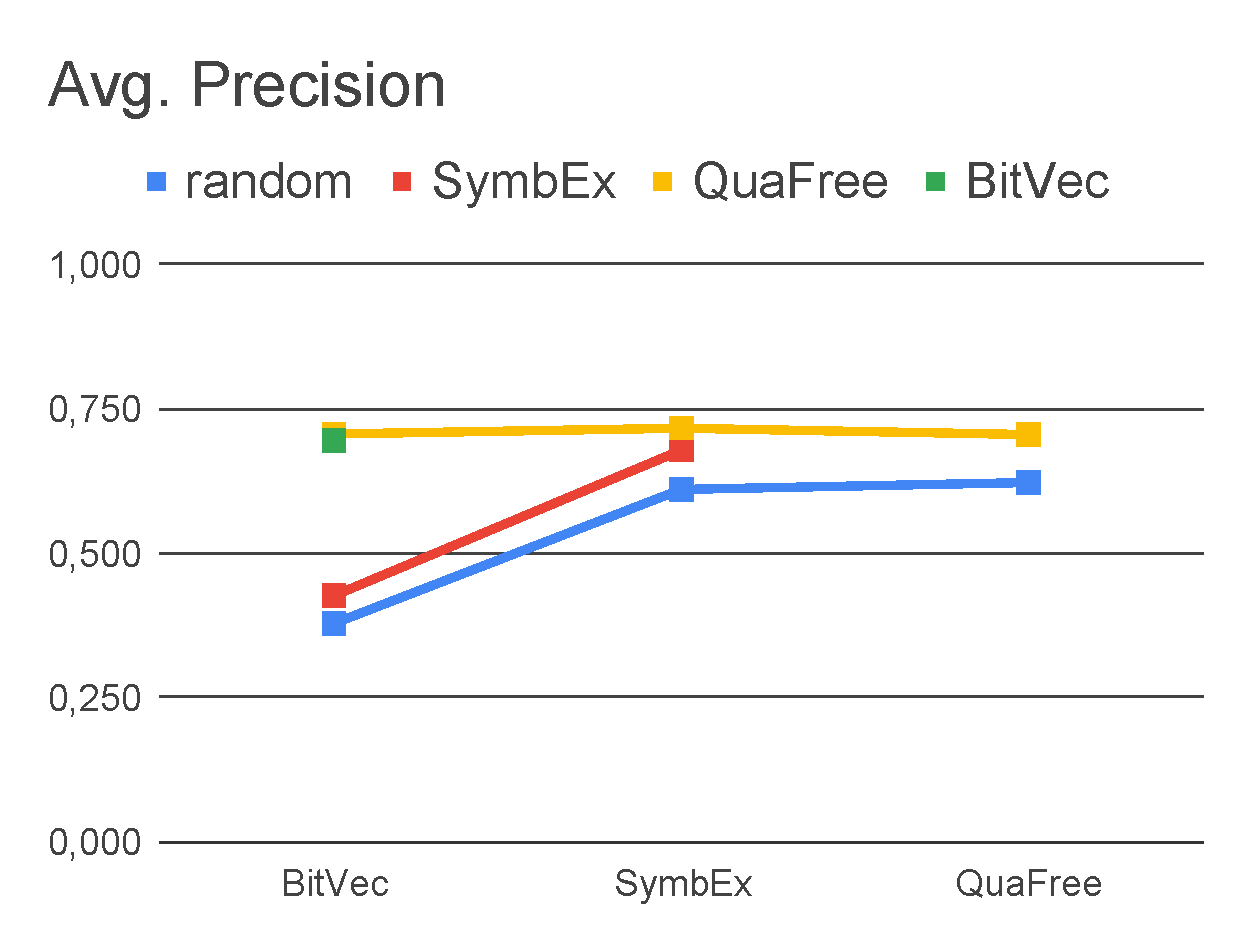
\includegraphics[scale=0.33]{./assets/smt-comp-ap.pdf}
\end{center}
\end{figure}

\end{minipage}
  
\end{frame}



\begin{frame}{Символьное исполнение}

\begin{center}
  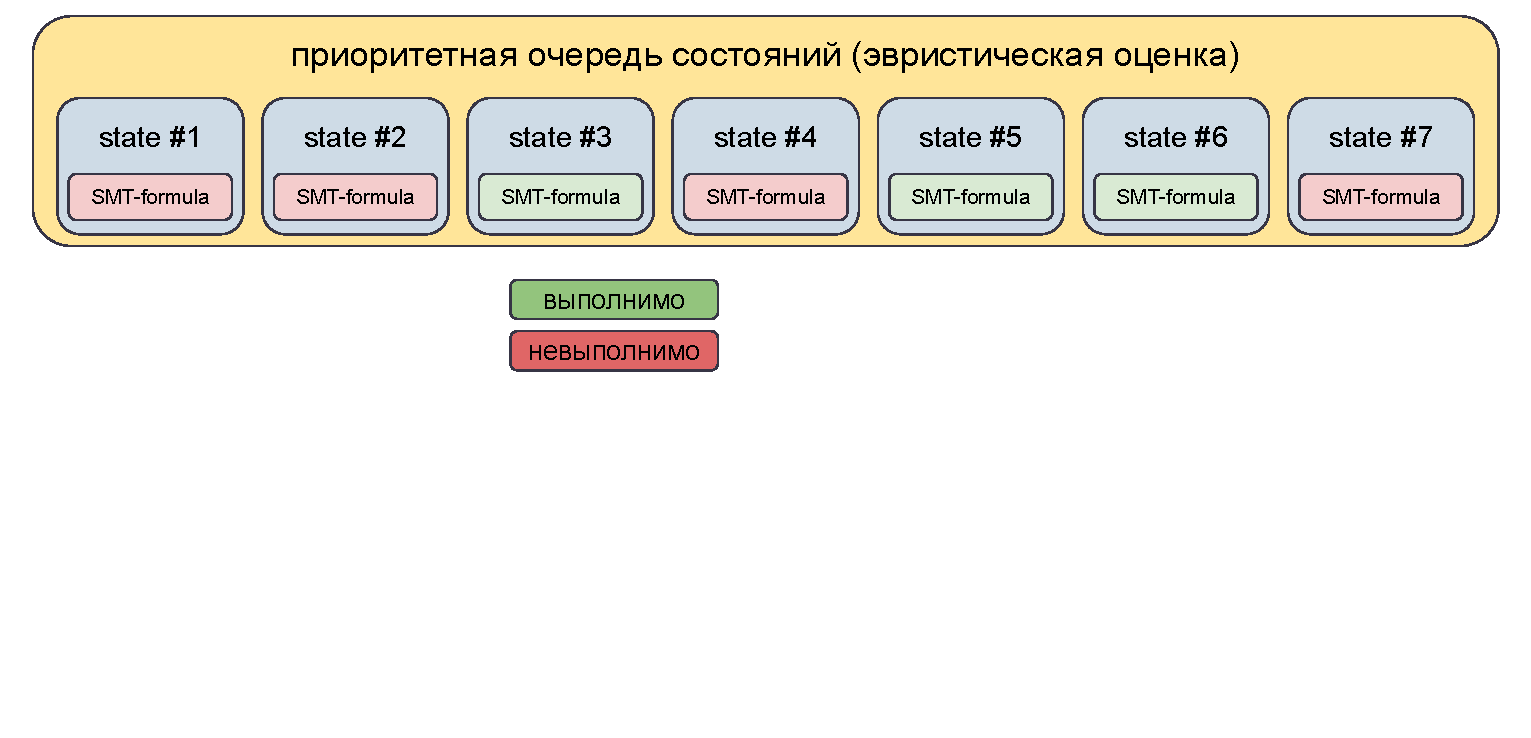
\includegraphics[scale=0.53]{./assets/symbex-ranking-1.pdf}
\end{center}

\end{frame}



\begin{frame}[noframenumbering]{Символьное исполнение}

\begin{center}
  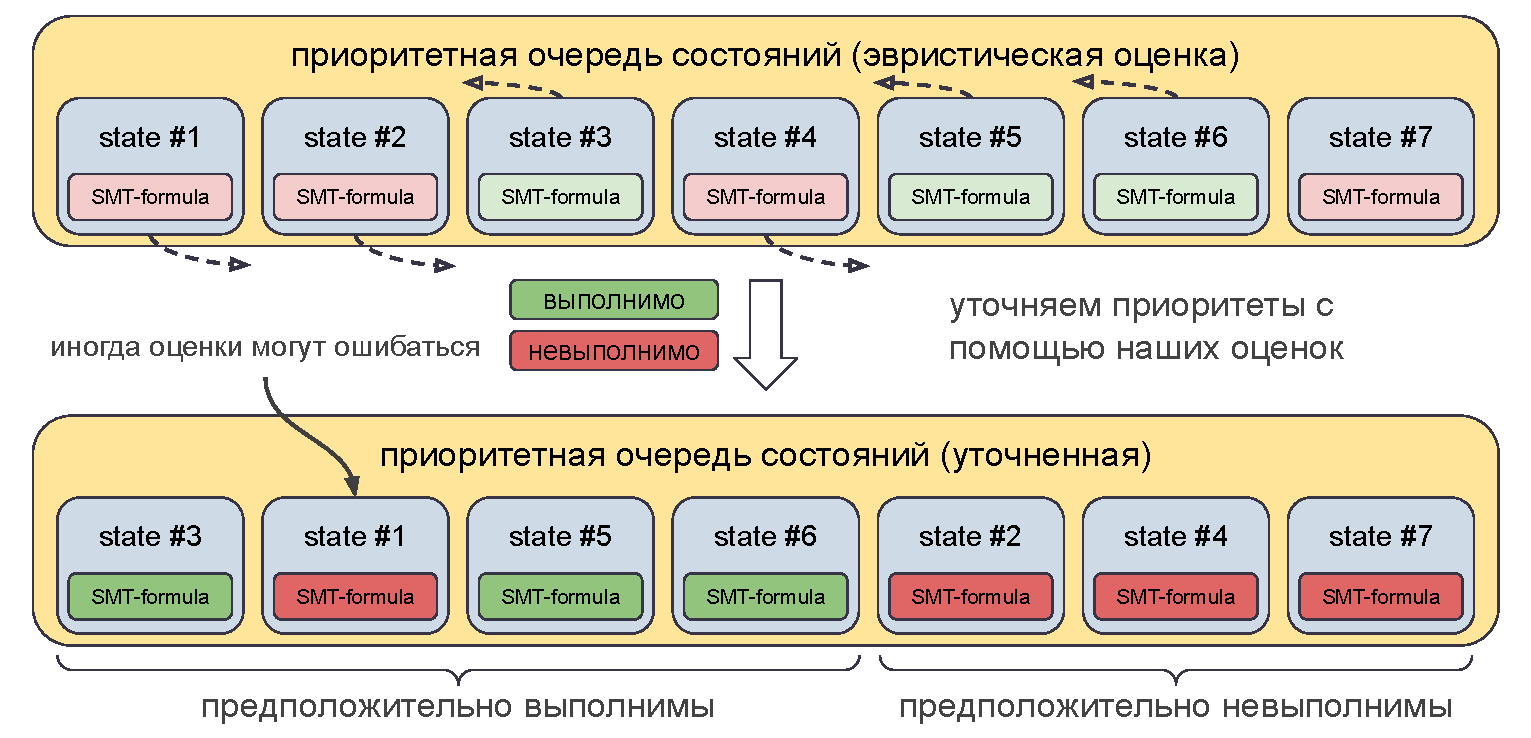
\includegraphics[scale=0.53]{./assets/symbex-ranking-2.pdf}
\end{center}

\end{frame}



\begin{frame}{Результаты SAGE Convolution (\texttt{USVM})}

\begin{minipage}{0.5\textwidth}

\begin{figure}[ht]
\begin{center}
  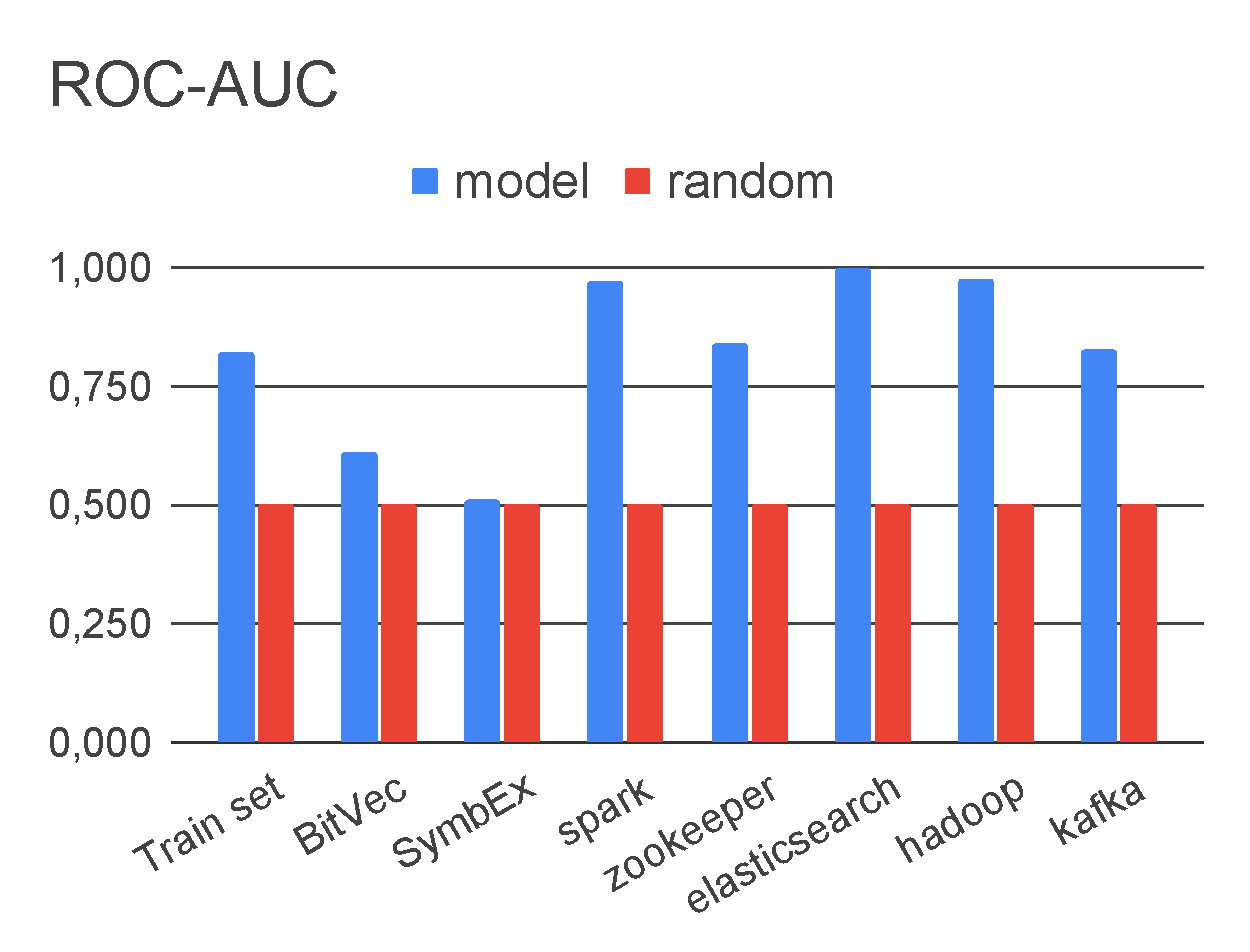
\includegraphics[scale=0.33]{./assets/usvm-roc-auc.pdf}
\end{center}
\end{figure}

\end{minipage}%
\begin{minipage}{0.5\textwidth}

\begin{figure}[ht]
\begin{center}
  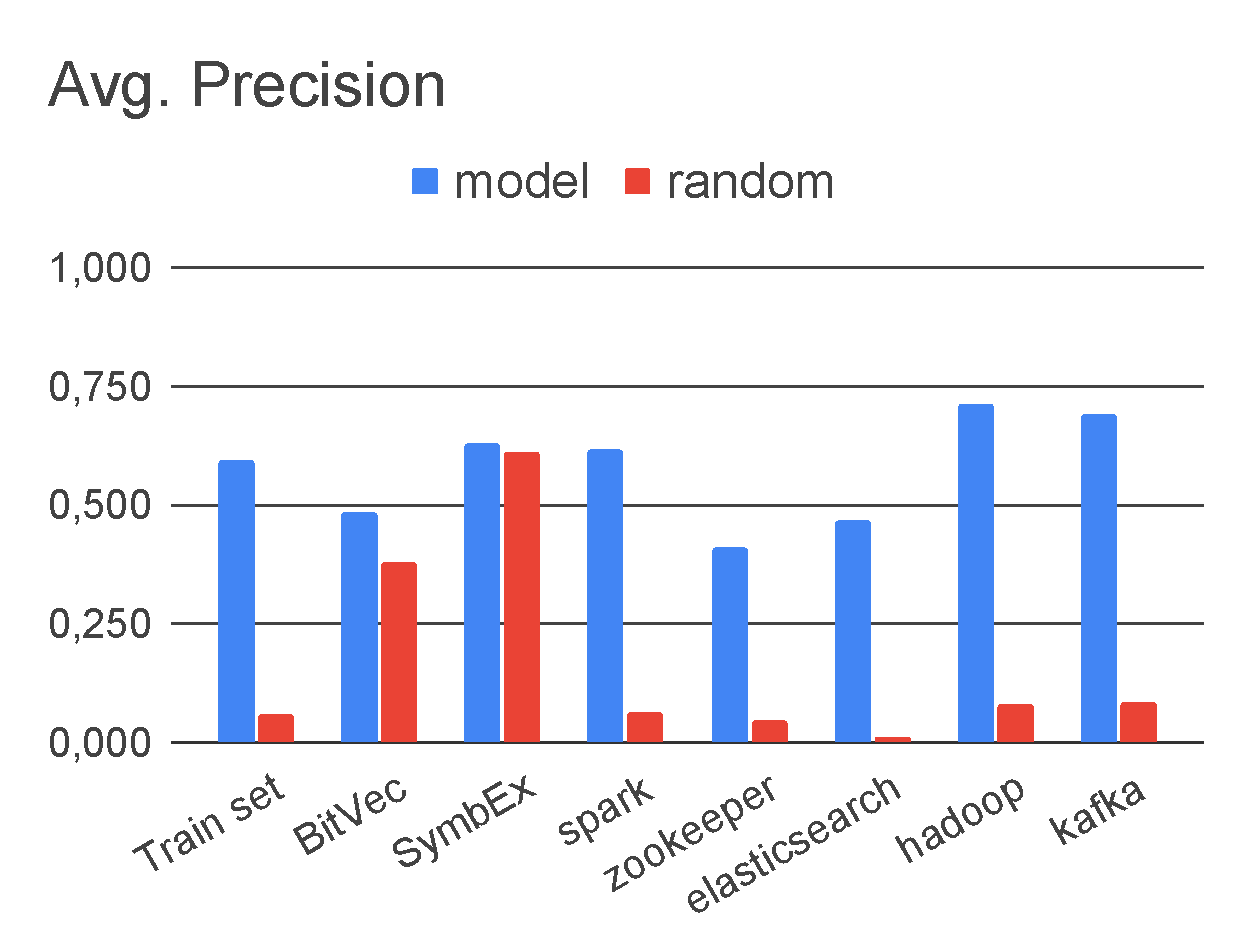
\includegraphics[scale=0.33]{./assets/usvm-ap.pdf}
\end{center}
\end{figure}

\end{minipage}

\end{frame}



\begin{frame}{Дальнейшее развитие}

\begin{itemize}
  \item Подбор гиперпараметров.
  \item Архитектурные улучшения.
  \item Аугментации данных.
  \item Постановка задачи ранжирования.
  \item Эффективная реализация и внедрение.
\end{itemize}

\end{frame}



\begin{frame}{Итоги работы}

\begin{enumerate}
  \item Спроектирована, обучена и протестирована первая нейросеть для предсказания выполнимости SMT-формул.
  \item Качество решения общей задачи плохое, но в случае одного из возможных практических применений результаты выглядят хорошо.
  \item Есть много идей для дальнейшего развития проекта.
\end{enumerate}

\vspace{2mm}\hrule

\begin{minipage}{0.5\textwidth}
\begin{center}

Степан Остапенко. tg: @flaax, \\ stepanos2002@gmail.com

\end{center}
\end{minipage}%
\begin{minipage}{0.5\textwidth}
\begin{center}


\includegraphics[scale=0.03]{./assets/booklet-qr.pdf}

{\small \url{https://qrco.de/bf9EBt}}

\end{center}
\end{minipage}

\end{frame}



\begin{frame}[noframenumbering, plain, allowframebreaks]{Источники}

\begin{thebibliography}{1}

\setbeamertemplate{bibliography item}[text]

\bibitem{smt-solver-working-scheme} SC$^{\text{2}}$: Satisfiability Checking Meets Symbolic Computation --- Scientific Figure on ResearchGate. Available from: \url{https://www.researchgate.net/figure/The-functioning-of-SMT-solvers_fig1_305214266} (дата обр. 11.06.2024).

\bibitem{smt-comp-2023-benchmarks} SMT-COMP 2023 benchmarks. URL: \url{https://smt-comp.github.io/2023/benchmarks.html} (дата обр. 20.05.2024).

\bibitem{usvm-github} USVM on github. URL: \url{https://github.com/UnitTestBot/usvm} (дата обр. 10.06.2024).

\bibitem{roc-auc-and-avg-prc} URL: \url{https://juandelacalle.medium.com/how-and-why-i-switched-from-the-roc-curve-to-the-precision-recall-curve-to-analyze-my-imbalanced-6171da91c6b8} (дата обр. 27.05.2024).

\bibitem{sage-conv-paper} William L. Hamilton et al. <<Inductive Representation Learning on Large Graphs>>.  \textit{ArXiv abs:1706.02216} (2017).

\bibitem{transformer-conv-paper} Yunsheng Shi et al. <<Masked Label Prediction: Unified Message Passing Model for Semi-Supervised Classification>>. \textit{ArXiv abs:2009.03509} (2021).

\bibitem{embeddings-for-numerical-features-paper} Yury Gorishniy, Ivan Rubachev and Artem Babenko. <<On Embeddings for Numerical Features in Tabular Deep Learning>>. \textit{Neural Information Processing Systems} (NeurIPS '2022).

\end{thebibliography}

\end{frame}



\begin{frame}[noframenumbering]{Параметры обучения}

\begin{table}[ht]
\begin{center}
\begin{tabular}{cc}
  \hline
  размерность эмбеддинга & 32 \\
  \hline
  функция потерь         & \textit{Cross-Entropy} \\
  оптимизатор            & \textit{AdamW} \\
  шаг обучения           & $10^{-4}$ \\
  штраф за веса          & $10^{-3}$ \\
  расписание             & \textit{Reduce LR On Plateau} \\
  \hline
  \texttt{val} выборка   & 15\% \\
  \texttt{test} выборка  & 10\% \\
  количество эпох        & 100
\end{tabular}
\end{center}
\end{table}

\end{frame}



\begin{frame}[noframenumbering]{Параметры датасетов с SMT-COMP}

\begin{table}[ht]
\begin{center}
\begin{tabular}{r|cccc}
  Датасет & \makecell{Количество \\ формул} & \makecell{Средний \\ размер \\ формулы} & \makecell{Средняя \\ глубина \\ формулы} & \makecell{Доля \\ выполнимых \\ формул} \\
  \hline \hline
  \rule{0pt}{2.5ex}
  \texttt{BitVec}  &  33\,797 & 1181.92 & 85.45 & 0.378 \\
  \texttt{SymbEx}  &  85\,078 &  669.46 & 49.24 & 0.610 \\
  \texttt{QuaFree} & 123\,396 &  965.16 & 48.71 & 0.622 \\
\end{tabular}
\caption{Параметры датасетов, полученных из данных с соревнования SMT-COMP~2023~\cite{smt-comp-2023-benchmarks}.}
\end{center}
\end{table}

\end{frame}



\begin{frame}[noframenumbering]{Параметры датасетов, собранных с USVM}

\begin{table}[ht]
\begin{center}
\begin{tabular}{r|cccc}
  Датасет & \makecell{Количество \\ формул} & \makecell{Средний \\ размер \\ формулы} & \makecell{Средняя \\ глубина \\ формулы} & \makecell{Доля \\ выполнимых \\ формул} \\
  \hline \hline
  \rule{0pt}{2.5ex}
  \texttt{u-test}  & 153\,778 & 522.84 &  5.18 & 0.038 \\
  \texttt{the-alg} & 181\,633 & 277.03 & 23.94 & 0.066 \\
  \texttt{u-core}  & 192\,744 & 179.42 & 12.19 & 0.066 \\
\end{tabular}
\caption{Параметры тренировочных датасетов, собранных в процессе работы символьного движка USVM \cite{usvm-github}.}
\end{center}
\end{table}

\end{frame}



\end{document}
